\subsection{Тематическое моделирование}
\subsubsection{Вероятностный латентный семантический анализ (pLSA)}
\par
Запишем плотность распределения выборки $\left(d_i, w_i\right)_{i=1}^{n}$:
\[\prod_{i=1}^{n} P(d_i, w_i) = \prod_{d\in D} \prod_{w\in d} P(d,w)^{n_{dw}},\]
что в сущности является функцией правдоподобия. Тогда максимизация логарифма правдоподобия запишется в виде:
\[\sum\limits_{d\in D}\sum\limits_{w\in d} n_{dw} \ln P(w|d)P(d) \to \max_{\Phi, \Theta},\]
где $P(d)$ -- константа, равная отношению длины документа на длину всей коллекции. В итоге имеем задачу математического программирования:
\[\sum\limits_{d\in D}\sum\limits_{w\in d} n_{dw} \ln\sum\limits_{t\in T} \phi_{wt}\theta_{td}\to \max_{\Phi, \Theta},\]
$\phi$ и $\theta$ -- параметры порождающей вероятностной модели. При ограничениях неотрицательности и нормировки, накладываемыми за счет аксиоматики Колмогорова:
\[\phi_{wt} \geq 0, \hspace*{0.3cm} \sum\limits_{w\in W} \phi_{wt} = 1; \hspace*{0.5cm} \theta_{td} \geq 0, \hspace*{0.3cm} \sum\limits_{t\in T} \theta_{td} = 1.\]
\bigskip\par
Из-за отсутствия корректной по Адамару постановки задачи в силу неединственности решения необходимо применить регуляризацию с целью доопределить решение дополнительными критериями.
%! расписать про неединственность решения
Максимизация логарифма правдоподобия с регуляризацией ARTM:
\[\sum\limits_{d,w} n_{dw} \ln \sum\limits_{t\in T} \phi_{wt}\theta_{td} + R(\Phi, \Theta) \to \max_{\Phi, \Theta}, \hspace*{0.3cm} R(\Phi, \Theta) = \sum\limits_{i} \tau_i R_i(\Phi, \Theta).\]
Для решения многокритериальной задачи математического программирования применяется метод простой итерации EM-алгоритм.
\bigskip\par
E-шаг:
\[p_{tdw} = P(t|d,w) = \underset{t\in T}{\mathrm{norm}}\left(\phi_{wt}\theta_{td}\right)\]
\bigskip\par
M-шаг:
\[\phi_{wt} = \underset{w\in W}{\mathrm{norm}} \left(n_{wt} + \phi_{wt}\dfrac{\partial R}{\partial \phi_{wt}}\right), \hspace*{0.3cm} n_{wt} = \sum\limits_{d\in D}n_{dw}p_{tdw}\]
\[\theta_{td} = \underset{t\in T}{\mathrm{norm}} \left(n_{td} + \theta_{td} \dfrac{\partial R}{\partial \theta_{td}}\right), \hspace*{0.3cm} n_{td} = \sum\limits_{w\in d} n_{dw} p_{tdw},\]
где $\underset{x\in X}{\mathrm{norm}} (y_x) = \dfrac{\max\left\{y_x, 0\right\}}{\sum\limits_{k\in X}\max\left\{x_k,0\right\}}.$
\bigskip\par
EM-алгоритм -- чередование шагов E и M до сходимости. При чем E-шаг есть условные вероятности тем $P(t|d, w)$, которые вычисляются через апостериорные вероятности $\phi_{wt}, \ \theta_{td}$ по формуле Байеса:
\[P(t|d,w) = \dfrac{P(w,t|d)}{P(w|d)} = \dfrac{P(w|t)P(t|d)}{P(w|d)} = \dfrac{\phi_{wt}\theta_{td}}{\sum\limits_{k}\phi_{wk}\theta_{kd}}.\]
M-шаг: при $R = 0$ частотные характеристики вычисляются суммированием $n_{tdw} = n_{dw} P(t|d, w)$:
\[\phi_{wt} = \dfrac{n_{wt}}{n_t}, \hspace*{0.3cm} n_{wt} = \sum\limits_{d\in D} n_{tdw}, \hspace*{0.3cm} n_t = \sum\limits_{w\in W} n_{wt}\]
\[\theta_{td} = \dfrac{n_{td}}{n_d}, \hspace*{0.3cm} n_{td} = \sum\limits_{w\in d} n_{tdw}, \hspace*{0.3cm} n_d = \sum\limits_{t\in T} n_{td}.\]
Для pLSA:
\[R(\Phi, \Theta) = 0.\]
M-шаг -- частотные оценки условных вероятностей:
\[\phi_{wt} = \underset{w\in W}{\mathrm{norm}}(n_{wt}), \hspace*{0.3cm} \theta_{td} = \underset{t\in T}{\mathrm{norm}}(n_{td}).\]
\subsubsection{Латентное размещение Дирихле (LDA)}
Регуляризация:
\[R(\Phi, \Theta) = \sum\limits_{t,w} \left(\beta_w - 1\right)\ln \phi_{wt} + \sum\limits_{d,t} \left(\alpha_t - 1\right) \ln\theta_{td}.\]
М-шаг -- сглаженные частотные характеристики с параметрами $\beta_w, \alpha_t$:
\[\phi_{wt} = \underset{w\in W}{\mathrm{norm}}(n_{wt} + \beta_w - 1), \hspace*{0.3cm} \theta_{td} = \underset{t\in T}{\mathrm{norm}}(n_{td} + \alpha_t - 1).\]
\textbf{Гипотеза}: Векторы $\phi_t = \left(\phi_{wt}\right)$ и $\theta_d = \left(\theta_{td}\right)$ порождаются распределениями Дирихле, причем $\alpha \in \mathbb{R}^{|T|}, \ \beta \in \mathbb{R}^{|W|}:$
\[\mathrm{Dir(\phi_t| \beta)} = \dfrac{\Gamma(\beta_0)}{\prod_{w\in W}\Gamma (\beta_w)} \prod_{w\in W} \phi_{wt}^{\beta_w-1}, \hspace*{0.3cm} \phi_{wt} > 0; \hspace*{0.3cm} \beta_0 = \sum\limits_{w \in W} \beta_w, \ \beta_t > 0;\]
\[\mathrm{Dir(\theta_d| \alpha)} = \dfrac{\Gamma(\alpha_0)}{\prod_{t\in T}\Gamma (\alpha_t)} \prod_{t\in T} \theta_{td}^{\alpha_t-1}, \hspace*{0.3cm} \theta_{td} > 0; \hspace*{0.3cm} \alpha_0 = \sum\limits_{t \in T} \alpha_t, \ \alpha_t > 0;\]
Запишем апостериорную вероятность для LDA:
\[\ln \prod_{d\in D} \prod_{w\in d} P(w,d | \Phi, \Theta)^{n_{dw}} = \prod_{t \in T}\mathrm{Dir}(\phi_t| \beta) \prod_{d\in D} \mathrm{Dir}(\theta_d|\alpha) \to \max_{\Phi, \Theta}\]
\begin{itemize}
    \item при $\beta_w > 1, \ \alpha_t > 1$ -- сглаживание;
    \item при $\beta \in (0,1), \ \alpha\in (0,1)$ -- слабое разреживание,
    \item при $\beta = \alpha = 1$ -- pLSA. 
\end{itemize}

\subsubsection{BERT Topic} 
Другим подходом к решению задачи тематического моделирования является кластеризация в векторном пространстве текстов с нейросетевой векторизацией текстов. Одной из самых актуальных моделей в решении поставленной задачи является BERTopic. Этапы работы алгоритма:
\begin{enumerate}
    \item Векторизация текстов (предобученные модели Bert Embeddings \cite{bert});
    \item Понижение размерности (методом UMAP \cite{leland});
    Во время работы алгоритм производит построение взвешенного графа, соединяя только те вершины, которые являются ближайшими соседями.\\ Пусть $X \in \mathbb{R}^n$ -- вершины графа (вектора слов в $n$-мерном пространстве). $T \in \mathbb{R}^{k}$ -- множество $k$-ближайших к $x_i \ \forall i$. Для каждого объекта рассчитывается расстояние до ближайшего соседа и величина $\sigma_i$ по формулам, соответственно:
    \[\rho_i = \min\limits_{t\in T} d(x_i, t),\]
    \[\sum\limits_{i}e^{-\left(\dfrac{d(x_i,y) - \rho_i}{\sigma_i}\right)} = \log_2 k\]
    Вес ребра, соединяющего $x_i$ и его соседа $t_k$ определяется по формуле:
    \[w_{ij} = e^{-\left(\dfrac{d(x_i, t_j) - \rho_i}{\sigma_i}\right)}.\] 
    Множество ребер построенного графа является нечетким с вероятностью существования ребра между двумя вершинами как функцией принадлежности. Вес ребра между двумя вершинами определяется по формуле:
    \[w_{x_i, x_j} = w(x_j \to x_i) + w(x_i \to x_j) - w(x_i \to x_j) \cdot w(x_j\to x_i).\] 
    Затем происходит построение графа в низкоразмерном пространстве и приближение его с исходным путем минимизации суммы дивергенций Кульбака-Лейблера для каждого из ребер $e$ из исходного и нового нечетких множеств:
    \[\sum\limits_{e \in E} w_h(e) \log \dfrac{w_h(e)}{w_l(e)} + (1-w_h(e))\log\left(\dfrac{1-w_h(e)}{1-w_l(e)}\right) \to \min\limits_{w_l},\]
    $w_h(e)$ -- функция принажлежности нечеткого множества из ребер в высокоразмерном пространстве, $w_l(e)$ -- функция принадлежности нечеткого множества из ребер в низкоразмерном пространстве. Задача оптимизации решается с помощью стохастического градиентного спуска.
    \item Кластеризация (метод HDBSCAN) \cite{clustering}:
    \begin{figure}[H]
        \centering
        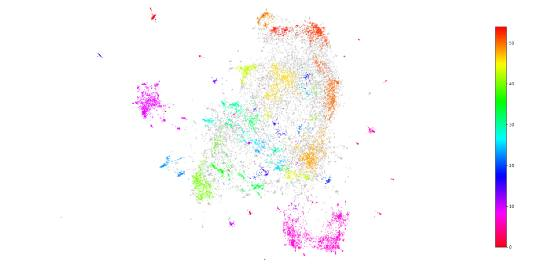
\includegraphics[scale=0.75]{hdbscan.jpg}
        \caption{Результат работы HDBSCAN}
        \label{fig:hdbscan}
    \end{figure}
\end{enumerate}
Формализуем HDBSCAN.
\begin{enumerate}
    \item Пусть $U_\epsilon(x)$ -- $\epsilon$-окрестность точки $x$, которая до этого не просматривалась. 
    \item Если точка $x$ содержит $minPts$ соседей (где $minPts$ и метрика, по которой находится расстояние между точками -- задаваемые гиперпараметры) или более, то образуется кластер
    \item Иначе точка помечается шумом. Возвращаемся к п.1.
    \item Повторяем, п.2-3 до момента, пока не получится связный кластер (между любыми соседями есть путь, как минимум, один);
    \item Повторяем п.1-4 для новой не просмотренной точки.
\end{enumerate}


